\documentclass[a4paper,oneside]{book}
\usepackage{listings}
\usepackage{amsmath}
\usepackage{listings}
\usepackage{epsfig}
\usepackage{color}
\definecolor{grayLines}{gray}{0.6}
\definecolor{grayText}{gray}{0.3}
\usepackage{multirow}
\usepackage{wasysym}
\usepackage{gensymb} 
\usepackage{longtable}

\setlength\parindent{0pt}
\begin{document}
\lstset{language=Python}          % Set your language (you can change the language for each code-block optionally)
\setcounter{secnumdepth}{3}
\setcounter{tocdepth}{3}
\tableofcontents

\newenvironment{paramFuncTable}
{\begin{center} 
\begin{longtable}{p{3.5cm}p{9cm}}
}
{\end{longtable} \end{center}}


\newenvironment{methodsTable}
{\begin{center}
\begin{longtable}{p{3.5cm}p{9cm}}
\multicolumn{2}{p{11cm}}{\color{grayText} \large{Methods}} \\
\multicolumn{2}{p{13cm}}{\color{grayLines} \rule{\linewidth}{0.25pt}} \\
\endfirsthead
\multicolumn{2}{p{11cm}}{\color{grayText} \large{Methods} \ldots continued from previous page} \\
\multicolumn{2}{p{13cm}}{\color{grayLines} \rule{\linewidth}{0.25pt}} \\
\endhead

\multicolumn{2}{p{13cm}}{\color{grayLines} \rule{\linewidth}{0.25pt}} \\
\multicolumn{2}{r}{{\color{grayText} continued on next page \ldots  }} \\ 
\endfoot

\endlastfoot

}
{\end{longtable} \end{center}}

\newenvironment{paramClassTable}
{\begin{center}
\begin{longtable}{lp{10cm}}
\multicolumn{2}{p{11cm}}{\color{grayText} \large{Parameters}} \\
\multicolumn{2}{p{13cm}}{\color{grayLines} \rule{\linewidth}{0.25pt}} \\
\endfirsthead
\multicolumn{2}{p{11cm}}{\color{grayText} \large{Parameters} \ldots continued from previous page} \\
\multicolumn{2}{p{13cm}}{\color{grayLines} \rule{\linewidth}{0.25pt}} \\
\endhead

\multicolumn{2}{p{13cm}}{\color{grayLines} \rule{\linewidth}{0.25pt}} \\
\multicolumn{2}{r}{{\color{grayText} continued on next page \ldots  }} \\ 
\endfoot

\endlastfoot
}
{\end{longtable} \end{center}}
 %environments definition
\newcommand{\A}[1]{{\tt A{#1}} & cross-sectional area of the section}
\newcommand{\alphaX}{{\tt alpha} & shear shape factor}
\newcommand{\alphaY}[1]{{\tt alphaY{#1}} & coefficient of distortion about the local y-axis}
\newcommand{\alphaZ}[1]{{\tt alphaZ{#1}} & coefficient of distortion about the local z-axis}
\newcommand{\bX}{{\tt b} & width}
\newcommand{\E}{{\tt E} & elastic modulus}
\newcommand{\Es}{{\tt Es} & elastic modulus}
\newcommand{\epsSMax}{{\tt epsSMax} & maximum strain in steel}
\newcommand{\epsCMin}{{\tt epsCMin} & minimum strain in concrete}
\newcommand{\EIy}[1]{{\tt EIy{#1}} & product of $E_{steel} \times I_y$ }
\newcommand{\EIz}[1]{{\tt EIz{#1}} & product of $E_{steel} \times I_z$} 
\newcommand{\eyd}[1]{{\tt eyd{#1}} & design strain at yield point}
\newcommand{\eyk}[1]{{\tt eyk{#1}} & characteristic strain at yield point}
\newcommand{\fmaxk}[1]{{\tt fmaxk{#1}} & characteristic value of the ultimate strength}
\newcommand{\fy}[1]{{\tt fy{#1}} &  yield strength}
\newcommand{\fyd}[1]{{\tt fyk{#1}} & design value of the yield strength}
\newcommand{\fyk}[1]{{\tt fyk{#1}} & characteristic value of the yield strength}
\newcommand{\fyn}[1]{{\tt fyn{#1}} &  stress at which material reaches plastic state in compression}
\newcommand{\fyp}[1]{{\tt fyp{#1}} & stress at which material reaches plastic state in tension}
\newcommand{\gammaS}{{\tt gammaS} & partial factor}
\newcommand{\G}[1]{{\tt G{#1}} & transverse modulus of elasticity}

\newcommand{\getAMzOne}{{\tt getAMz1} & returns the bending moment about the local Z axis applied to the back end of the element}
\newcommand{\getAMzTwo}{{\tt getAMz2} & returns the bending moment about the local Z axis applied to the front end of the element}
\newcommand{\getANTwo}{{\tt getAN2} & returns the axial force applied to the front end of the element}
\newcommand{\getAVyOne}{{\tt  getAVy1} & returns the shear force in local Y axis appliend on the back end of the element}
\newcommand{\getAVyTwo}{{\tt  getAVy2} & returns the shear force in local Y axis direction applied on the front end of the element}
\newcommand{\getAVzOne}{{\tt  getAVz1} & returns the shear force in local Z axis appliend on the back end of the element}
\newcommand{\getAVzTwo}{{\tt  getAVz2} & returns the shear force in local Z axis direction applied on the front end of the element}

\newcommand{\getMOne}{{\tt getM1} & returns the bending moment at the back end of the element}
\newcommand{\getMTwo}{{\tt getM2} & returns the bending moment at the front end of the element}
\newcommand{\getMyOne}{{\tt getMy1} & returns the bending moment about the local Y axis at the back end of the element}
\newcommand{\getMyTwo}{{\tt  getMy2} &  returns the bending moment  about the local Y axis at the front end of the element}
\newcommand{\getMzOne}{{\tt getMz1} & returns the bending moment about the local Z axis at the back end of the element}
\newcommand{\getMzTwo}{{\tt  getMz2} &  returns the bending moment  about the local Z axis at the front end of the element}

\newcommand{\getN}{{\tt getN} & returns the mean value of the axial force at the the element $N=\cfrac{N_1 + N_2}{2}$}
\newcommand{\getNOne}{{\tt getN1} & returns the axial force at the back end of the element}
\newcommand{\getNTwo}{{\tt getN2} & returns the axial force at the front end of the element}
\newcommand{\getT}{{\tt getT} & returns the mean value of the torsional moment at the the element }
\newcommand{\getTOne}{{\tt getT1} & returns the torsional moment at the back end of the element}
\newcommand{\getTTwo}{{\tt getT2} & returns the torsional moment at the front end of the element}
\newcommand{\getV}{{\tt getV} & returns the shear force at the central section of the element}
\newcommand{\getVDirEjeFuerteLocales}{{\tt getVDirEjeFuerteLocales()} & returns a vector, expressed in local coordinates, that defines the strong axis orientation}
\newcommand{\getVDirEjeDebilLocales}{{\tt getVDirEjeDebilLocales()} & returns a vector, expressed in local coordinates, that defines the weak axis orientation}
\newcommand{\getAnguloEjeFuerte}{{\tt getAnguloEjeFuerte()} & returns the angle between the strong axis and the plane XZ of the element}
\newcommand{\getAnguloEjeDebil}{{\tt getAnguloEjeDebil()} & returns the angle between the weak axis and the plane XZ of the element}
\newcommand{\getVDirEjeFuerteGlobales}{{\tt getVDirEjeFuerteGlobales()} & returns a vector, expressed in global coordinates, that defines the strong axis orientation}
\newcommand{\getVDirEjeDebilGlobales}{{\tt getVDirEjeDebilGlobales()} & returns a vector, expressed in global coordinates, that defines the weak axis orientation}

\newcommand{\getVOne}{{\tt getV1} & returns the shear force at the back end of the element}
\newcommand{\getVTwo}{{\tt getV2} & returns the shear force at the front end of the element}
\newcommand{\getVy}{{\tt getVy} & returns the element mean shear force in the local Y axis direction}
\newcommand{\getVyOne}{{\tt  getVy1} & returns the shear force in local Y axis direction at the back end of the element}
\newcommand{\getVyTwo}{{\tt  getVy2} & returns the shear force in local Y axis direction at the front end of the element}
\newcommand{\getVz}{{\tt getVz} & returns the element mean shear force in the local Z axis direction}
\newcommand{\getVzOne}{{\tt  getVz1} & returns the shear force in local Z axis direction at the back end of the element}
\newcommand{\getVzTwo}{{\tt  getVz2} & returns the shear force in local Z axis direction at the front end of the element}

\newcommand{\GJ}[1]{{\tt GJ{#1}} & product of $E_{steel} \times G$ }
\newcommand{\h}{{\tt h} & height}
\newcommand{\IAxisOne}[1]{{\tt I1{#1}} &  second moment of area about the axis through the centre of gravity and parallel to the width dimension (axis 1)}
\newcommand{\iAxisOne}[1]{{\tt i1{#1}} & bending radius of the section with regard to the axis 1}
\newcommand{\IAxisTwo}[1]{{\tt I2{#1}} &  second moment of area about the axis through the centre of gravity and parallel to the high dimension (axis 2)}
\newcommand{\iAxisTwo}[1]{{\tt i2{#1}} & bending radius of the section with regard to the axis 2}
\newcommand{\initialStrain}{{\tt initialStrain} & initial strain in the element}
\newcommand{\Iy}[1]{{\tt Iy{#1}} &  second moment of area about the local y-axis}

\newcommand{\Iz}[1]{{\tt Iz{#1}} &  second moment of area about the local z-axis}
\newcommand{\J}[1]{{\tt J{#1}} & torsional moment of inertia of the section }
\newcommand{\M}{{\tt M} & bending moment}
\newcommand{\mdlr}{{\tt mdlr} & modeler name}
\newcommand{\MeAxisOne}[1]{{\tt Me1{#1}} & yield moment of the rectangular section about the axis 1}
\newcommand{\N}{{\tt N} & axial force}
\newcommand{\name}[1]{{\tt name} & name identifying the {#1}}
\newcommand{\nDivIJ}{{\tt nDivIJ} & number of cells in IJ (width) direction}
\newcommand{\numDivIJ}{{\tt numDivIJ} & number of cells in IJ (width) direction}
\newcommand{\nDivJK}{{\tt nDivJK} & number of cells in JK  (height) direction}
\newcommand{\numDivJK}{{\tt numDivJK} & number of cells in JK  (height) direction}
\newcommand{\nuX}{{\tt nu} & Poisson's ratio}
\newcommand{\rhoX}{{\tt rho} &  mass density}
\newcommand{\V}{{\tt V} & shear force}
\newcommand{\Wyel}[1]{{\tt Wyel{#1}} & elastic section modulus about the local y-axis}
\newcommand{\Wzel}[1]{{\tt Wzel()} & elastic section modulus about the local z-axis}

%Elements variables
\newcommand{\ElementParam}
{
%{\tt getNodes} & \\ 
{\tt getIdxNodes} & vector containing the node index to be used in Vtk graphics \\
{\tt getDimension} & element dimension \\
{\tt getVtkCellType} & cell type for Vtk graphics\\ 
}

\newcommand{\ElementMeth}
{
{\tt commitState()} & the element is to commit its current state; returns $0$ if successful, a negative number if not\\
{\tt revertToLastCommit()} & the element is to set its current state to the last committed state; returns $0$ if successful, a negative number if not\\
{\tt revertToStart} & the element is to set its current state to the state it was at before the analysis started; returns $0$ if successful, a negative number if not\\
{\tt getNumDOF} & returns the number of DOF associated with the element; this should equal the sum of the DOFs at each of the external nodes \\
{\tt getResistingForce()} & returns the resisting force vector for the element; this is equal to the applied load due to element loads minus the loads at the nodes due to internal stresses in the element due to the current trial displacement, i.e. $ R_e = P_{e} - f_{R_e}(U_{trial}) $ \\ 
{\tt setDeadSRF} & assigns Stress Reduction Factor for element deactivation\\ 
{\tt getVtkCellType()} & returns cell type for Vtk graphics\\ 
{\tt getMEDCellType()} & returns cell type for MED file writing.\\
\multicolumn{2}{l}{{\tt getPosCentroid(geomInicial)}}\\
 & returns the element centroid position. \\
& {\tt geomInicial = True} to consider the initial geometry shape \\
& {\tt geomInicial = False} to consider the deformed geometry shape \\
\multicolumn{2}{l}{{\tt getCooCentroid(geomInicial)}} \\
 & returns the element centroid coordinates\\ 
& {\tt geomInicial = True} to consider the initial geometry shape \\
& {\tt geomInicial = False} to consider the deformed geometry shape \\
\multicolumn{2}{l}{{\tt getPoints(ni,nj,nk,geomInicial)}}\\
 & returns a uniform grid of points over the element.\\ 
& {\tt ni,nj,nk} number of divisions in i,j,k directions \\
& {\tt getLongTributaria} \emph{True} to consider the initial geometry shape, \emph{False} for the deformed geometry shape\\
{\tt resetTributarias()} & reset the tributary length, area and volume of connected nodes \\
{\tt vuelcaTributarias} & \\
\multicolumn{2}{l}{{\tt calculaLongsTributarias(geomInicial)}} \\
 & returns the tributary length associated with each node of the element; the parameter {\tt geomInicial = True} to consider the initial geometry shape in the calculation or {\tt geomInicial = False} for the deformed geometry shape\\
\multicolumn{2}{l}{{\tt getLongTributaria(Node)}} \\
 & returns the tributary length associated with the {\tt Node} given as argument\\
\multicolumn{2}{l}{{\tt getLongTributariaByTag(tag)}}\\
 & returns the tributary length associated with the node labelled with the {\tt tag} given as argument \\
\multicolumn{2}{l}{{\tt calculaAreasTributarias(geomInicial)}}\\
 & returns the tributary area associated with each node of the element; the parameter {\tt geomInicial = True} to consider the initial geometry shape in the calculation or {\tt geomInicial = False} for the deformed geometry shape\\
\multicolumn{2}{l}{{\tt getAreaTributaria(Node)}} \\
 & returns the tributary area associated with the {\tt Node} given as argument\\
\multicolumn{2}{l}{{\tt getAreaTributariaByTag(tag)}} \\
& returns the tributary area associated with the node labelled with the {\tt tag} given as argument \\
\multicolumn{2}{l}{{\tt calculaVolsTributarios(geomInicial)}} \\
 & returns the tributary volume associated with each node of the element; the parameter {\tt geomInicial = True} to consider the initial geometry shape in the calculation or {\tt geomInicial = False} for the deformed geometry shape\\
\multicolumn{2}{l}{{\tt getVolTributario(Node)}} \\
 & returns the tributary volume associated with the {\tt Node} given as argument\\
\multicolumn{2}{l}{{\tt getVolTributarioByTag(tag)}} \\
& returns the tributary volume associated with the node labelled with the {\tt tag} given as argument \\
{\tt getMaxCooNod(axisIdx)} & returns the maximum value among the coordinates in the {\tt axisIdx} axis of the external nodes associated with the element ({\tt axisIdx} adopts the values {\tt 0,1,}\ldots) \\
{\tt getMinCooNod(axisIdx)} & returns the minimum value among the coordinates in the {\tt axisIdx} axis of the external nodes associated with the element ({\tt axisIdx} adopts the values {\tt 0,1,}\ldots)\\
}


\newcommand{\ElementZERODParam}
{
{\tt getIVector} & vector in the element local x-axis direction\\
{\tt getJVector} & vector in the element local y-axis direction\\
{\tt getKVector} & vector in the element local z-axis direction\\
}

\newcommand{\ElementZERODMeth}
{
{\tt setupVectors(x,yp)} & establish orientation of element for the transformation matrix \\
& {\tt x} vector in global coordinates defining local x-axis \\
& {\tt yp} vector in global coordinates which lies in the local x-y plane for the element \\
& local z-axis is defined by the vector $\vec{z}=\vec{x}\times\vec{yp}$ \\
}

\newcommand{\ElementOneDParam}
{
{\tt getCoordTransf()} & returns the identifier of the coordinate-transformation associated with the element\\
}

\newcommand{\ElementOneDMeth}
{
{\tt getMEDCellType()} &  interface with MED data format for Salome\\
\multicolumn{2}{l}{{\tt vector2dUniformLoadGlobal(v)}} \\
 & applies a uniform surface load to the element; the value and direction of the load is defined by the 2D vector $\vec{v}$, expressed in the global coordinate system  \\
\multicolumn{2}{l}{{\tt vector2dUniformLoadLocal(v)}} \\
 & applies a uniform surface load to the element; the value and direction of the load is defined by the 2D vector $\vec{v}$, expressed in the element local coordinate system \\
\multicolumn{2}{l}{{\tt vector2dPointByRelDistLoadGlobal(d,v)}} \\
 &  applies a punctual force to the element; scalar $d$ specifies the offset distance from node 2 (toward node 1) where the force is applied, this distance is input as a length fraction (its value varies between 0 and 1); 2D vector $\vec{v}$ defines the force value and orientation, its coordinates are expressed in the global system\\
\multicolumn{2}{l}{{\tt vector2dPointByRelDistLoadLocal(d,v)}} \\
 &  applies a punctual force to the element; scalar $d$ specifies the offset distance from node 2 (toward node 1) where the force is applied, this distance is input as a length fraction (its value varies between 0 and 1); 2D vector $\vec{v}$ defines the force value and orientation, its coordinates are expressed in the element local system\\
\multicolumn{2}{l}{{\tt vector2dPointLoadGlobal(p,v)}} \\
 &  applies a punctual force to the element;  2D vector $\vec{p}$ defines the global coordinates of the point of application of the force; 2D vector $\vec{v}$ defines the force value and orientation (in global coordinates) \\
\multicolumn{2}{l}{{\tt vector2dPointLoadLocal(p,v)}} \\
 &  applies a punctual force to the element;  2D vector $\vec{p}$ defines the coordinates of the point of application of the force; 2D vector $\vec{v}$ defines the force value and orientation; both vectors are expressed in the element local-coordinate system \\
\multicolumn{2}{l}{{\tt vector3dUniformLoadGlobal(v)}} \\
 &  applies a uniform surface load to the element; the value and direction of the load is defined by the 3D vector $\vec{v}$, expressed in the global coordinate system\\
\multicolumn{2}{l}{{\tt vector3dUniformLoadLocal(v)}} \\
 &  applies a uniform surface load to the element; the value and direction of the load is defined by the 3D vector $\vec{v}$, expressed in the element local coordinate system\\
\multicolumn{2}{l}{{\tt vector3dPointByRelDistLoadGlobal(d,v)}} \\
 &  applies a punctual force to the element; scalar $d$ specifies the offset distance from node 2 (toward node 1) where the force is applied, this distance is input as a length fraction (its value varies between 0 and 1); 3D vector $\vec{v}$ defines the force value and orientation, its coordinates are expressed in the global system\\
\multicolumn{2}{l}{{\tt vector3dPointByRelDistLoadLocal(d,v)}} \\
 & applies a punctual force to the element; scalar $d$ specifies the offset distance from node 2 (toward node 1) where the force is applied, this distance is input as a length fraction (its value varies between 0 and 1); 3D vector $\vec{v}$ defines the force value and orientation, its coordinates are expressed in the element local-coordinate system \\
\multicolumn{2}{l}{{\tt vector3dPointLoadGlobal(p,v)}} \\
 & applies a punctual force to the element;  3D vector $\vec{p}$ defines the global coordinates of the point of application of the force; 3D vector $\vec{v}$ defines the force value and orientation (in global coordinates)\\
\multicolumn{2}{l}{{\tt vector3dPointLoadLocal(p,v)}} \\
 &  applies a punctual force to the element;  3D vector $\vec{p}$ defines the coordinates of the point of application of the force; 3D vector $\vec{v}$ defines the force value and orientation; both vectors are expressed in the element local-coordinate system \\
\multicolumn{2}{l}{{\tt strainLoad(PlanoDeformacion1,PlanoDeformacion2)}} \\
 &  This function creates an imposed strain load in the current load case. The first argument defines the deformation at element start and the second at the element's end.\\
{\tt getCooPuntos(ndiv)} & returns $ndiv-1$ equally-spaced points on the element\\
}

\newcommand{\ProtoTrussMeth}
{
{\tt getDim()} &  returns element dimension \\
{\tt getMaterial()} &  returns the material associated with the element \\
}

\newcommand{\ProtoBeamTwoDParam}
{
{\tt sectionProperties} & \\
}

\newcommand{\ProtoBeamThreeDParam}
{
{\tt sectionProperties} & \\
}

\newcommand{\BeamColumnWithSectionFDMeth}
{
{\tt getNumSections} & \\
{\tt getSections} & Returns element sections\\
}

\newcommand{\TrussBaseMeth}
{
{\tt getL} & returns the element length \\
}




\newcommand{\ZeroLengthMeth}
{
{\tt clearMaterials()} & clears all material definition of the element \\
\multicolumn{2}{l}{{\tt setMaterial(dir,matName)}} \\
 & assigns uni-axial materials to the different directions of the element\\
& {\tt dir}: integer representing the direction in which the uni-axial material acts: {\tt dir} is 0,1,2 for translation in the local x, y, z axes or 3, 4, 5 
for rotation about the local x, y, z axes.\\
& {\tt matName}: string representing the name of the material \\
{\tt getMaterials} &  \\
}


\newcommand{\ZeroLengthSectionMeth}
{
{\tt getSection()} & returns the section axial force-deformation associated with the element \\
{\tt getMaterial()} & returns the section axial force-deformation associated with the element \\
}

\newcommand{\MuelleMeth}
{
{\tt getN} & Returns the internal axial force $N$ in the element\\
}

\newcommand{\TrussMeth}
{
{\tt area} &  cross-sectional area of the element\\
{\tt getN} &  Returns the internal axial force $N$ in the element \\
}

\newcommand{\CorotTrussParam}
{
{\tt area} &  cross-sectional area of the element\\
}
\newcommand{\CorotTrussMeth}
{
{\tt getN} &  RReturns the internal axial force $N$ in the element \\
}

  %Latex variables definition

\chapter{Finite element model components}

\section{Nodes}

\subsection{Description}
The nodes of a finite element mesh are the points where the degrees of freedom reside. Each node object has, at least, the following information:

\begin{itemize}
\item Coordinates wich define its position in space. Typically (x,y,z) coordinates.
\item Definition of the degrees of freedom in the node (displacements, rotations,\ldots)
\end{itemize}

The nodes can also serve to define loads or masses that act over the model at its position.

\subsection{Node creation}

To create a node you can use the following commands:

\begin{lstlisting}[frame=single]
  nodos.newNodeXY(x,y)
  nodos.newNodeIDXY(tag,x,y)
  nodos.newNodeXYZ(x,y,z)
  nodos.newNodeIDXYZ(x,y,z)
\end{lstlisting}

\noindent where:

\begin{description}
\item{nodos:} is a node container obtained from the preprocessor.
\item{tag:} is an integer that identifies the node in the model.
\item{(x,y) or (x,y,z):} are the cartesian coordinates that define node's position.
\end{description}

\subsection{Predefined spaces}
Nodes definition in typical elastic FE models.
\begin{verbatim}
from model import predefined_spaces as ps
nodos= preprocessor.getNodeLoader
\end{verbatim}
\begin{center} 
\begin{longtable}{ll}
{\tt ps.gdls\_elasticidad2D(nodos)} & 2 node coordinates $(x,y)$ \\
                                    & 2 node DOF $(u_x,u_y)$ \\ 
{\tt ps.gdls\_resist\_materiales2D(nodos)} & 2 node coordinates $(x,y)$ \\
                                    & 3 node DOF $(u_x,u_y,\theta)$ \\ 
{\tt ps.gdls\_elasticidad3D(nodos)} & 3 node coordinates $(x,y,z)$ \\
                                    & 3 node DOF $(u_x,u_y,u_z)$ \\ 
{\tt ps.gdls\_resist\_materiales3D(nodos)} & 3 node coordinates $(x,y)$ \\
                                    & 6 node DOF $(u_x,u_y,u_z,\theta_x,\theta_y,\theta_z)$ \\ 
\end{longtable} \end{center}



\section{Constraints}
\subsection{MP constraints}

\subsubsection{Description}
An MP\_Constraint represents a multiple point constraint in the domain. A multiple point constraint imposes a relationship between the displacement for certain dof at two nodes in the model, typically called the {\em retained} node and the {\em constrained} node:

\begin{equation}
U_c = C_{cr} U_r
\end{equation}


An MP\_Constraint is responsible for providing information on the relationship between the dof, this is in the form of a constraint matrix, $C_{cr}$, and two ID objects, {\em retainedID} and {\em constrainedID} indicating the dof's at the nodes represented by $C_{cr}$. For example, for the following constraint imposing a relationship between the displacements at node $1$, the constrained node, with the displacements at node $2$, the retainednode in a problem where the x,y,z components are identified as the 0,1,2 degrees-of-freedom:

\begin{align}
u_{1,x} &= 2 u_{2,x} + u_{2,z} \\
u_{1,y} &= 3 u_{2,z}
\end{align}

\noindent the constraint matrix is:

\begin{equation}
C_{cr} =
\left[
\begin{array}{cc}
2 & 1  \\
0 & 3
\end{array}
\right] 
\end{equation}

\noindent and the vectors defining the dof's at the nodes are:

\begin{align}
constrainedID &= [0, 1] \\
retainedID &= [0, 2]
\end{align}



\chapter{Solver components}

\section{Analysis components}
\subsection{Constraints}

\subsubsection{LagrangeMP\_FE}
LagrangeMP\_FE is a subclass of FE\_Element used to enforce a
multi point constraint, of the form $U_c = C_{cr} U_r$, where $U_c$ are
the constrained degrees-of-freedom at the constrained node, $U_r$ are
the retained degrees-of-freedom at the retained node and $C_{cr}$ a
matrix defining the relationship between these degrees-of-freedom. 

To enforce the constraint the following are added to the tangent and
the residual:
\[ \left[ \begin{array}{cc} 0 & \alpha C^t \\ \alpha C & 0 \end{array}
\right] ,
\left\{ \begin{array}{c} 0 \\ 0 \end{array} \right\} \]

\noindent at the locations
corresponding to the constrained degree-of-freedoms specified by the
MP\_Constraint, i.e. $[U_c$ $U_r]$, and the lagrange multiplier
degrees-of-freedom introduced by the LagrangeConstraintHandler for
this constraint, $C = [-I$ $ C_{cr}]$. Nothing is added to the residual. \\  


To construct a LagrangeMP\_FE element to enforce the constraint
specified by the MP\_Constraint {\em theMP} using a default value for
$\alpha$ of $alpha$. The FE\_Element class constructor is called with
the integers $3$ and the two times the size of the {\em retainedID}
plus the size of the {\em constrainedID} at the MP\_Constraint {\em
theMP} plus . A Matrix and a Vector object are created for adding the
contributions to the tangent and the residual. The residual is
zeroed. If the MP\_Constraint is not time varying, then the contribution to the
tangent is determined. Links are set to the retained and constrained
nodes. The DOF\_Group tag ID is set using the tag of the constrained
Nodes DOF\_Group, the tag of the retained Node Dof\_group and the tag
of the LagrangeDOF\_Group, {\em theGroup}. A warning message is printed and 
the program is terminated if either not enough memory is available for
the Matrices and Vector or the constrained and retained Nodes of their
DOF\_Groups do not exist. \\




\indent {\em virtual void setID(void);} \\
Causes the LagrangeMP\_FE to determine the mapping between it's equation
numbers and the degrees-of-freedom. This information is obtained by
using the mapping information at the DOF\_Group objects associated with
the constrained and retained nodes and the LagrangeDOF\_Group, {\em
theGroup}. Returns $0$ if
successful. Prints a warning message and returns a negative number if
an error occurs: $-2$ if the
Node has no associated DOF\_Group, $-3$ if the constrained DOF
specified is invalid for this Node (sets corresponding ID component to
$-1$ so nothing is added to the tangent) and $-4$ if the ID in the
DOF\_Group is too small for the Node (again setting corresponding ID
component to $-1$). \\ 

\indent {\em virtual const Matrix \&getTangent(Integrator *theIntegrator);} \\
If the MP\_Constraint is time-varying, from the MP\_Constraint
{\em theMP} it obtains the current $C_{cr}$ matrix; it then adds the
contribution to the tangent matrix. Returns this tangent Matrix.

\indent {\em virtual const Vector \&getResidual(Integrator *theIntegrator);} \\
Returns the residual, a $zero$ Vector. \\




\chapter{Materials and sections}
\section{Stardard uniaxial materials}
\subsection{defElasticMaterial}
\noindent Construct an elastic uniaxial material
\begin{verbatim}
defElasticMaterial(mdlr,name,E)
\end{verbatim}
\vspace{-10pt}
{\color{grayLines} \rule{\linewidth}{0.25pt}}
\begin{center}
\begin{tabular}{lp{10cm}}
{\tt mdlr} & modeler name \\
{\tt name} & name identifying the material \\
{\tt E} & tangent in the stress-strain diagram (see figure \ref{Elastic}) \\
\end{tabular}
\end{center}
\paragraph{Example}
\begin{verbatim}
*
\end{verbatim}

\begin{figure}[h]
\centering
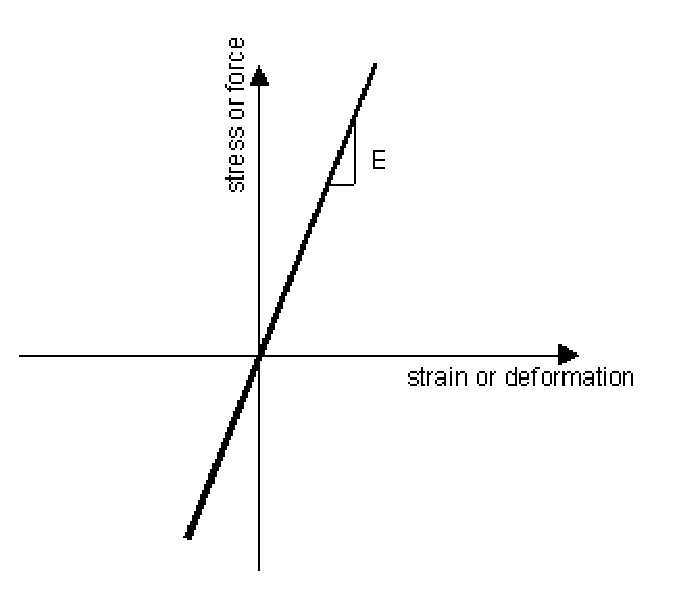
\includegraphics[width=60mm]{materials/figures/Elastic}
\caption{Elastic uniaxial material. Stress-strain diagram}\label{Elastic}
\end{figure}

\subsection{defElasticPPMaterial}
\noindent Construct an elastic perfectly-plastic uniaxial material
\begin{verbatim}
defElasticPPMaterial(mdlr,name,E,fyp,fyn)
\end{verbatim}
\vspace{-10pt}
{\color{grayLines} \rule{\linewidth}{0.25pt}}
\begin{center}
\begin{tabular}{lp{10cm}}
{\tt mdlr} & modeler name \\
{\tt name} & name identifying the material \\
{\tt E} & tangent in the elastic zone of the stress-strain diagram (see figure \ref{ElasticPP}) \\
{\tt fyp} & stress at which material reaches plastic state in tension (see figure \ref{ElasticPP}) \\
{\tt fyn} &  stress at which material reaches plastic state in compression (see figure \ref{ElasticPP}) \\
{\tt } &  \\
\end{tabular}
\end{center}
\paragraph{Example}
\begin{verbatim}
*
\end{verbatim}

\begin{figure}[h]
\centering
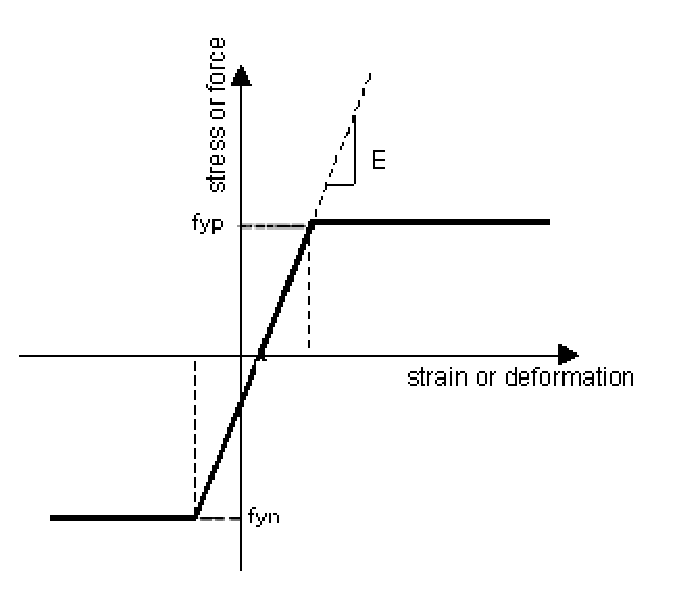
\includegraphics[width=60mm]{materials/figures/ElasticPP}
\caption{Elastic perfectly-plastic uniaxial material. Stress-strain diagram}\label{ElasticPP}
\end{figure}

\subsection{defElastNoTracMaterial}
\noindent Construct a uniaxial elastic-no tension material
\begin{verbatim}
defElastNoTracMaterial(mdlr,name,E)
\end{verbatim}
\vspace{-10pt}
{\color{grayLines} \rule{\linewidth}{0.25pt}}
\begin{center}
\begin{tabular}{lp{10cm}}
{\tt mdlr} & modeler name \\
{\tt name} & name identifying the material \\
{\tt E} & tangent in the elastic zone of the stress-strain diagram (see figure \ref{ENT}) \\
\end{tabular}
\end{center}
\paragraph{Example}
\begin{verbatim}
*
\end{verbatim}
\begin{figure}[h]
\centering
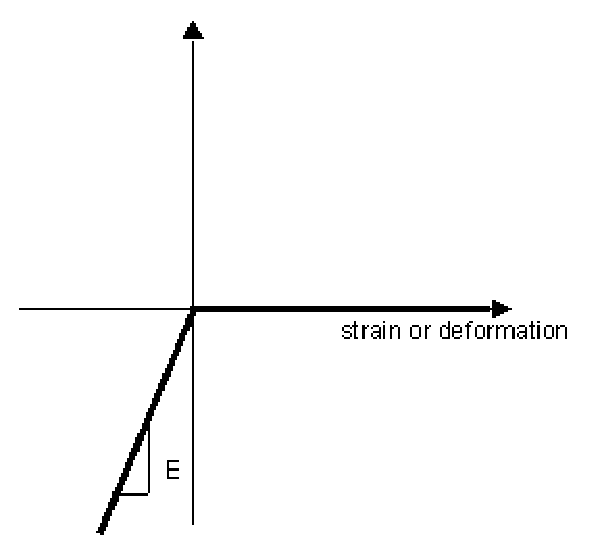
\includegraphics[width=50mm]{materials/figures/ENT}
\caption{Elastic-no tension material. Stress-strain diagram}\label{ENT}
\end{figure}

\section{Steel and reinforcing steel materials}
\subsection{defCableMaterial}
\noindent Construct a uniaxial bilinear prestressed material. The stress strain ranges from slack (large strain at zero stress) to taught (linear with modulus E).
\begin{verbatim}
defCableMaterial(mdlr,name,E,prestress,rho)
\end{verbatim}
\vspace{-10pt}
{\color{grayLines} \rule{\linewidth}{0.25pt}}
\begin{center}
\begin{tabular}{lp{10cm}}
{\tt mdlr} & modeler name \\
{\tt name} & name identifying the material \\
{\tt E} & Young modulus \\
{\tt prestress} & prestress \\
{\tt rho} & effective self weight (gravity component of weight per volume transverse to the cable) \\
\end{tabular}
\end{center}
\paragraph{Example}
\begin{verbatim}
*
\end{verbatim}


\subsection{defSteel01}
\noindent Construct a uniaxial bilinear steel material object with kinematic hardening
\begin{verbatim}
defSteel01(mdlr,name,E,fy,b)
\end{verbatim}
\vspace{-10pt}
{\color{grayLines} \rule{\linewidth}{0.25pt}}
\begin{center}
\begin{tabular}{lp{10cm}}
{\tt mdlr} & modeler name \\
{\tt name} & name identifying the material \\
{\tt E} & initial elastic tangent (see figure \ref{Steel01}) \\
{\tt fy} &  yield strength (see figure \ref{Steel01})\\
{\tt b} &  strain-hardening ratio: ratio between post-yield tangent and initial elastic tangent (see figure \ref{Steel01})\\
\end{tabular}
\end{center}
\paragraph{Example}
\begin{verbatim}
*
\end{verbatim}

\begin{figure}[h]
\centering
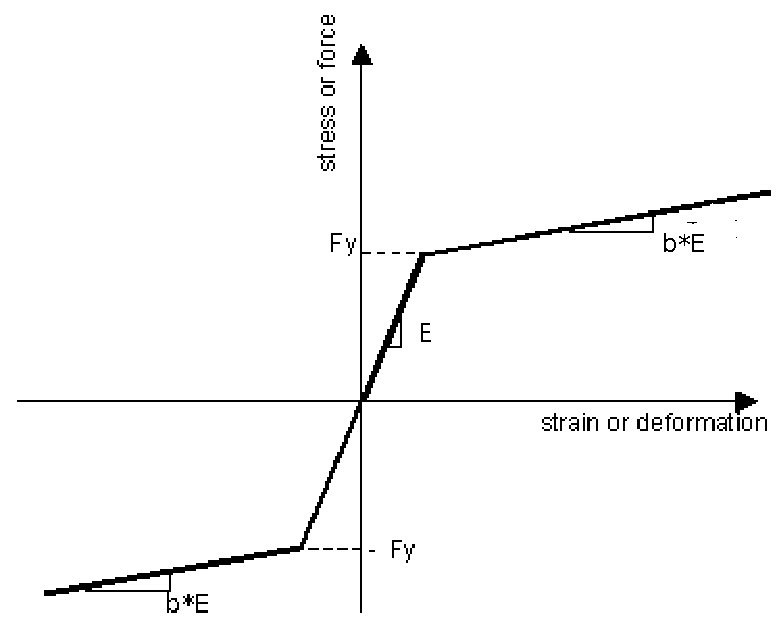
\includegraphics[width=60mm]{materials/figures/Steel01}
\caption{Steel001: uniaxial bilinear steel material with kinematic hardening. Stress-strain diagram}\label{Steel01}
\end{figure}


\subsection{defSteel02}
\noindent Construct a uniaxial Giuffre-Menegotto-Pinto steel material object with isotropic strain hardening
\begin{verbatim}
defSteel02(mdlr,name,E,fy,b,initialStress)
\end{verbatim}
\vspace{-10pt}
{\color{grayLines} \rule{\linewidth}{0.25pt}}
\begin{center}
\begin{tabular}{lp{10cm}}
{\tt mdlr} & modeler name \\
{\tt name} & name identifying the material \\
{\tt E} & initial elastic tangent (see figure \ref{Steel02}) \\
{\tt fy} &  yield strength (see figure \ref{Steel02})\\
{\tt b} &  strain-hardening ratio: ratio between post-yield tangent and initial elastic tangent)\\
{\tt initialStress} &  initial stress \\
\end{tabular}
\end{center}
{\footnotesize The transition from elastic to plastic branches  (see figure \ref{Steel02}) is controlled by parameters R0, R1, R2. The default values R0=15, R1=0.925 and R2=0.15}
\paragraph{Example}
\begin{verbatim}
*
\end{verbatim}

\begin{figure}[h]
\centering
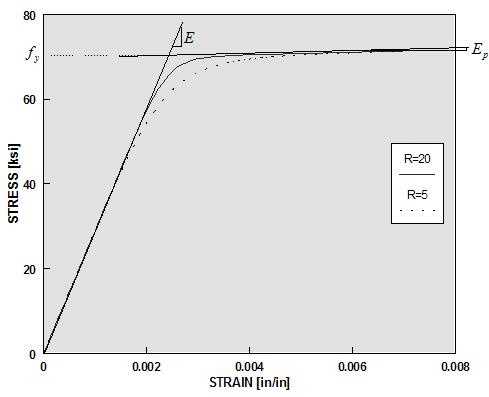
\includegraphics[width=60mm]{materials/figures/Steel02Monotonic}
\caption{Steel002: uniaxial bilinear steel material with isotropic strain hardening. Stress-strain diagram}\label{Steel02}
\end{figure}

\subsection{ReinforcingSteel}
\noindent This class constructs a bilinear stress-strain diagram to carry out the analysis of reinforced concrete according to Eurocode 2. Other national standards, like the spanish EHE and the swiss SIA also adopt this diagram.

\begin{center}
\begin{tabular}{lp{10cm}}
\multicolumn{2}{p{11cm}}{\color{grayText} \large{Parameters}} \\
\multicolumn{2}{p{13cm}}{\color{grayLines} \rule{\linewidth}{0.25pt}} \\
{\tt nmbMaterial} & name identifying the material \\
{\tt nmbDiagK} & name identifying the characteristic stress-strain diagram (default: {\tt "dgK"+nmbMaterial}) \\
{\tt tagDiagK} & tag of the uniaxial material with the characteristic stress-strain diagram\\
{\tt nmbDiagD} &  name identifying the design stress-strain diagram (default: {\tt "dgD"+nmbMaterial}) \\
{\tt tagDiagD} & tag of the uniaxial material with the design stress-strain diagram\\
{\tt fyk} & characteristic value of the yield strength\\
{\tt gammaS} & partial factor for material (default: 1.15)\\
{\tt Es} & elastic modulus of the material (default: 2e11)\\
{\tt emax} & maximum strain at failure point\\
{\tt k} & ratio between characteristic ultimate stress and characteristic yield stress $^{(1)}$ (default: 1.05)\\
\multicolumn{2}{p{13cm}}{\color{grayLines} \rule{\linewidth}{0.25pt}} \\
\multicolumn{2}{p{13cm}}{\footnotesize{(1): according to annex C of EC2: for class A k$\ge$1,05, for class B k$\ge$1,08}}
\end{tabular}
\end{center}

\begin{center}
\begin{tabular}{lp{9cm}}
\multicolumn{2}{p{11cm}}{\color{grayText} \large{Methods}} \\
\multicolumn{2}{p{13cm}}{\color{grayLines} \rule{\linewidth}{0.25pt}} \\
{\tt fmaxk()} & characteristic ultimate strength \\
{\tt fyd()} & design yield stress \\
{\tt eyk()} & characteristic strain at yield point\\
{\tt eyd()} & design strain at yield point\\
{\tt Esh()} &  post-yield tangent\\
{\tt bsh()} & ratio between post-yield tangent and initial elastic tangent\\
{\tt defDiagK(mdlr)} & returns XC uniaxial material (characteristic values)\\
{\tt defDiagD(mdlr)} & returns XC uniaxial material (design values)\\
\end{tabular}
\end{center}

\section{Concrete materials}
\subsection{defConcrete01}
\noindent Construct a uniaxial Kent-Scott-Park concrete material object with degraded linear unloading/reloading stiffness according to the work of Karsan-Jirsa and no tensile strength.
\begin{verbatim}
defConcrete01(mdlr,name,epsc0,fpc,fpcu,epscu)
\end{verbatim}
\vspace{-10pt}
{\color{grayLines} \rule{\linewidth}{0.25pt}}
\begin{center}
\begin{tabular}{lp{10cm}}
{\tt mdlr} & modeler name \\
{\tt name} & name identifying the material \\
{\tt fpc} &  concrete compressive strength at 28 days (compression is negative) $^{(1)}$\\
{\tt epsc0} &  concrete strain at maximum strength (see figure \ref{Concrete01}) $^{(2)}$\\
{\tt fpcu} &  concrete crushing strength (see figure \ref{Concrete01}) \\
{\tt epscu} &  concrete strain at crushing strength (see figure \ref{Concrete01}) \\
\hline
\multicolumn{2}{p{12cm}}{\footnotesize(1): Compressive concrete parameters should be input as negative values (if input as positive, they will be converted to negative internally)}\\
\multicolumn{2}{p{12cm}}{\footnotesize (2): The initial slope for this model is $2*fpc/epsc0$ (see figure \ref{Concrete01})}\\
\end{tabular}
\end{center}
\paragraph{Example}
\begin{verbatim}
*
\end{verbatim}

\begin{figure}[h]
\centering
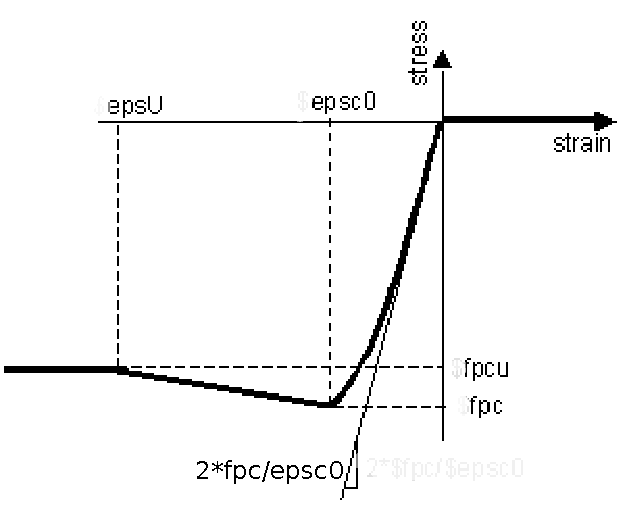
\includegraphics[width=60mm]{materials/figures/Concrete01}
\caption{Concrete01: uniaxial Kent-Scott-Park concrete material. Stress-strain diagram}\label{Concrete01}
\end{figure}

\section{ND materials}
An ND material is an object that represents the stress-strain relationship at the gauss-point of a continuum element.

\subsection{defElasticIsotropic3d}
\noindent Construct an elastic isotropic material.
\begin{verbatim}
defElasticIsotropic3d(mdlr,name,E,nu,rho)
\end{verbatim}
\vspace{-10pt}
{\color{grayLines} \rule{\linewidth}{0.25pt}}
\begin{center}
\begin{tabular}{lp{10cm}}
{\tt mdlr} & modeler name \\
{\tt name} & name identifying the material\\
{\tt E} & elastic modulus \\
{\tt nu} & Poisson's ratio \\
{\tt rho} &  mass density, optional (default = 0.0)\\
\end{tabular}
\end{center}
\paragraph{Example}
\begin{verbatim}
*
\end{verbatim}

\subsection{defElasticIsotropicPlaneStrain}
\noindent Construct an elastic isotropic plane-strain material.
\begin{verbatim}
defElasticIsotropicPlaneStrain(mdlr,name,E,nu,rho)
\end{verbatim}
\vspace{-10pt}
{\color{grayLines} \rule{\linewidth}{0.25pt}}
\begin{center}
\begin{tabular}{lp{10cm}}
{\tt mdlr} & modeler name \\
{\tt name} & name identifying the material\\
{\tt E} & elastic modulus \\
{\tt nu} & Poisson's ratio \\
{\tt rho} &  mass density, optional (default = 0.0)\\
\end{tabular}
\end{center}
\paragraph{Example}
\begin{verbatim}
*
\end{verbatim}

\subsection{defElasticIsotropicPlaneStress}
\noindent Construct an elastic isotropic plane-stress material.
\begin{verbatim}
defElasticIsotropicPlaneStress(mdlr,name,E,nu,rho)
\end{verbatim}
\vspace{-10pt}
{\color{grayLines} \rule{\linewidth}{0.25pt}}
\begin{center}
\begin{tabular}{lp{10cm}}
{\tt mdlr} & modeler name \\
{\tt name} & name identifying the material\\
{\tt E} & elastic modulus \\
{\tt nu} & Poisson's ratio \\
{\tt rho} &  mass density, optional (default = 0.0)\\
\end{tabular}
\end{center}
\paragraph{Example}
\begin{verbatim}
*
\end{verbatim}
\section{Sections}
A section represents a force-deformation (or resultant stress-strain) relationship at beam-column or plate element.

Three types of sections are going to be considered:
\begin{description}
\item{Elastic:} defined by material and geometric constants;
\item{Resultant:} general nonlinear description of force-deformation response, e.g. moment-curvature;
\item{Fiber:} section is discretized into smaller regions for which the material stress-strain response is integrated to give resultant behavior, e.g. reinforced concrete.
\end{description}
\subsection{Elastic sections}
\subsubsection{defElasticSection2d}
\noindent Construct an elastic section appropiate for 2D beam analysis.
\begin{verbatim}
defElasticSection2d(mdlr,name,A,E,I)
\end{verbatim}
\vspace{-10pt}
{\color{grayLines} \rule{\linewidth}{0.25pt}}
\begin{center}
\begin{tabular}{lp{10cm}}
{\tt mdlr} & modeler name \\
{\tt name} & name identifying the section \\
{\tt A} &  cross-sectional area of the section \\
{\tt E} &  Young's modulus of material \\
{\tt I} &  second moment of area about the local z-axis\\
\end{tabular}
\end{center}
\paragraph{Example}
\begin{verbatim}
*
\end{verbatim}


\subsubsection{defElasticShearSection2d}
\noindent Construct an elastic section appropiate for 2D beam analysis, including shear deformations.
\begin{verbatim}
defElasticShearSection2d(mdlr,name,A,E,G,I,alpha)
\end{verbatim}
\vspace{-10pt}
{\color{grayLines} \rule{\linewidth}{0.25pt}}
\begin{center}
\begin{tabular}{lp{10cm}}
{\tt mdlr} & modeler name \\
{\tt name} & name identifying the section \\
{\tt A} &  cross-sectional area of the section \\
{\tt E} &  Young's modulus of material \\
{\tt G} & shear modulus \\
{\tt I} &  second moment of area about the local z-axis\\
{\tt alpha} & shear shape factor \\
\end{tabular}
\end{center}
\paragraph{Example}
\begin{verbatim}
*
\end{verbatim}

\subsubsection{defElasticSectionFromMechProp2d}
\noindent Construct an elastic section appropiate for 2D beam analysis, taking mechanical properties of the section form a MechProp2d object.
\begin{verbatim}
defElasticSectionFromMechProp2d(mdlr,name,mechProp2d)
\end{verbatim}
\vspace{-10pt}
{\color{grayLines} \rule{\linewidth}{0.25pt}}
\begin{center}
\begin{tabular}{lp{10cm}}
{\tt mdlr} & modeler name \\
{\tt name} & name identifying the section \\
{\tt mechProp2d} & object that contains mechanical properties of the section  \\
\end{tabular}
\end{center}
\paragraph{Example}
\begin{verbatim}
*
\end{verbatim}

%%%
\subsubsection{defElasticSection3d}
\noindent Construct an elastic section appropiate for 3D beam analysis.
\begin{verbatim}
defElasticSection3d(mdlr,name,A,E,G,Iz,Iy,J)
\end{verbatim}
\vspace{-10pt}
{\color{grayLines} \rule{\linewidth}{0.25pt}}
\begin{center}
\begin{tabular}{lp{10cm}}
{\tt mdlr} & modeler name \\
{\tt name} & name identifying the section \\
{\tt A} &  cross-sectional area of the section \\
{\tt E} &  Young's modulus of material \\
{\tt Iz} &  second moment of area about the local z-axis\\
{\tt Iy} &  second moment of area about the local y-axis\\
{\tt J} & torsional moment of inertia of the section \\
\end{tabular}
\end{center}
\paragraph{Example}
\begin{verbatim}
*
\end{verbatim}


\subsubsection{defElasticShearSection3d}
\noindent Construct an elastic section appropiate for 3D beam analysis, including shear deformations.
\begin{verbatim}
defElasticShearSection3d(mdlr,name,A,E,G,Iz,Iy,J,alpha)
\end{verbatim}
\vspace{-10pt}
{\color{grayLines} \rule{\linewidth}{0.25pt}}
\begin{center}
\begin{tabular}{lp{10cm}}
{\tt mdlr} & modeler name \\
{\tt name} & name identifying the section \\
{\tt A} &  cross-sectional area of the section \\
{\tt E} &  Young's modulus of material \\
{\tt G} & shear modulus \\
{\tt Iz} &  second moment of area about the local z-axis\\
{\tt Iy} &  second moment of area about the local y-axis\\
{\tt J} & torsional moment of inertia of the section \\
{\tt alpha} & shear shape factor \\
\end{tabular}
\end{center}
\paragraph{Example}
\begin{verbatim}
*
\end{verbatim}

\subsubsection{defElasticSectionFromMechProp3d}
\noindent Construct an elastic section appropiate for 3D beam analysis, taking mechanical properties of the section form a MechProp3d object.
\begin{verbatim}
defElasticSectionFromMechProp3d(mdlr,name,mechProp3d)
\end{verbatim}
\vspace{-10pt}
{\color{grayLines} \rule{\linewidth}{0.25pt}}
\begin{center}
\begin{tabular}{lp{10cm}}
{\tt mdlr} & modeler name \\
{\tt name} & name identifying the section \\
{\tt mechProp3d} & object that contains mechanical properties of the section  \\
\end{tabular}
\end{center}
\paragraph{Example}
\begin{verbatim}
*
\end{verbatim}

\subsubsection{defElasticMembranePlateSection}
\noindent Construct an an isotropic elastic section appropriate for plate and shell analysis.
\begin{verbatim}
defElasticMembranePlateSection(mdlr,name,E,nu,rho,h)
\end{verbatim}
\vspace{-10pt}
{\color{grayLines} \rule{\linewidth}{0.25pt}}
\begin{center}
\begin{tabular}{lp{10cm}}
{\tt mdlr} & modeler name \\
{\tt name} & name identifying the section\\
{\tt E} &  Young's modulus\\
{\tt nu} &  Poisson's modulus\\
{\tt rho} &  mass density\\
{\tt h} &  depth of section\\
\end{tabular}
\end{center}
\paragraph{Example}
\begin{verbatim}
*
\end{verbatim}

\subsubsection{defElasticPlateSection}
\noindent Construct an an isotropic elastic section appropriate for plate analysis.
\begin{verbatim}
defElasticPlateSection(mdlr,name,E,nu,rho,h)
\end{verbatim}
\vspace{-10pt}
{\color{grayLines} \rule{\linewidth}{0.25pt}}
\begin{center}
\begin{tabular}{lp{10cm}}
{\tt mdlr} & modeler name \\
{\tt name} & name identifying the section\\
{\tt E} &  Young's modulus\\
{\tt nu} &  Poisson's modulus\\
{\tt rho} &  mass density\\
{\tt h} &  depth of section\\
\end{tabular}
\end{center}
\paragraph{Example}
\begin{verbatim}
*
\end{verbatim}

\subsection{Fiber sections}
\subsubsection{FiberSet}
\noindent This class constructs a set of fibers for a fiber section
\begin{verbatim}
FiberSet(scc,nmbSet,tagDiag)
\end{verbatim}
\begin{center}
\begin{tabular}{lp{10cm}}
\multicolumn{2}{p{11cm}}{\color{grayText} \large{Parameters}} \\
\multicolumn{2}{p{13cm}}{\color{grayLines} \rule{\linewidth}{0.25pt}} \\
{\tt scc} & name identifying the fiber section \\
{\tt nmbSet} & name of the set of fibers to be generated \\
{\tt tagDiag} & tag of the uniaxial material which forms the fibers \\
\end{tabular}
\end{center}

\begin{center}
\begin{tabular}{lp{9cm}}
\multicolumn{2}{p{11cm}}{\color{grayText} \large{Methods}} \\
\multicolumn{2}{p{13cm}}{\color{grayLines} \rule{\linewidth}{0.25pt}} \\
{\tt getFiberWithMinStrain()} & returns the fiber of the set that has the minimum strain \\
{\tt getFiberWithMaxStrain()} & returns the fiber of the set that has the maximum strain \\
\end{tabular}
\end{center}


\subsubsection{RCSets}
\noindent This class constructs the sets (concrete and reinforcing steel) of a reinforced concrete fiber section.
\begin{verbatim}
RCSets(scc,tagCdiag, nmbSetC,tagSdiag, nmbSetS)
\end{verbatim}
\begin{center}
\begin{tabular}{lp{10cm}}
\multicolumn{2}{p{11cm}}{\color{grayText} \large{Parameters}} \\
\multicolumn{2}{p{13cm}}{\color{grayLines} \rule{\linewidth}{0.25pt}} \\
{\tt scc} & name identifying the fiber section \\
{\tt tagCDiag} & tag of the uniaxial material that makes up the concrete fibers of the section \\
{\tt nmbSetC} & name of the set of fibers of concrete to be generated \\
{\tt tagSdiag} & tag of the uniaxial material that makes up the reinforcing steel fibers of the section \\
{\tt nmbSetS} & name of the set of fibers of reinforcing steel to be generated \\
\end{tabular}
\end{center}

\begin{center}
\begin{tabular}{lp{9cm}}
\multicolumn{2}{p{11cm}}{\color{grayText} \large{Methods}} \\
\multicolumn{2}{p{13cm}}{\color{grayLines} \rule{\linewidth}{0.25pt}} \\
{\tt reselTractionFibers(scc,tractionFibersSetName)} & returns the set of fibers in tension \\
{\tt getConcreteArea(factor)} & returns the concrete area \\
{\tt getMaxConcreteStrain()} & returns the maximum strain in the set of concrete fibers \\
{\tt getConcreteInitialTangent()} & returns the initial tangent in the stress-strain diagram of material that makes up the fibers of concrete \\
{\tt getConcreteCompression()} & returns the resultant of compressive stresses in concrete fibers \\
{\tt getNumBarrasTraccion()} & returns the number of reinforcing steel fibers in tension \\
\end{tabular}
\end{center}

\subsubsection{fiberSectionSetupRCSets}
Returns an object of the class \verb|RCSets|
\begin{verbatim}
fiberSectionSetupRCSets(scc,tagCdiag, nmbSetC,tagSdiag, nmbSetS)
\end{verbatim}
\vspace{-10pt}
{\color{grayLines} \rule{\linewidth}{0.25pt}}
\begin{center}
\begin{tabular}{lp{10cm}}
{\tt scc} & name identifying the fiber section \\
{\tt tagCdiag} & tag of the uniaxial material that makes up the concrete fibers of the section \\
{\tt nmbSetC} & name of the set of fibers of concrete to be generated \\
{\tt tagSdiag} & tag of the uniaxial material that makes up the reinforcing steel fibers of the section \\
{\tt nmbSetS} & name of the set of fibers of reinforcing steel to be generated \\
\end{tabular}
\end{center}

\subsubsection{creaSetsFibrasHA}
Construct the sets of concrete fibers (\verb|"hormigon"|) and reinforcing steel fibers (\verb|"armadura"|) for all the elements included in a set of elements.
\begin{verbatim}
creaSetsFibrasHA(mdlr, nmbSet, tagHA, tagAcero)
\end{verbatim}
\vspace{-10pt}
{\color{grayLines} \rule{\linewidth}{0.25pt}}
\begin{center}
\begin{tabular}{lp{10cm}}
{\tt mdlr} & modeler name \\
{\tt nmbSet} & name identifying the set of elements \\
{\tt tagHA} & tag of the uniaxial material that makes up the concrete fibers of the section \\
{\tt tagAcero} & tag of the uniaxial material that makes up the reinforcing steel fibers of the section \\
\end{tabular}
\end{center}

\subsubsection{reselTractionFibers}
Returns the fibers under tension included in a set of fibers.
\begin{verbatim}
reselTractionFibers(scc,fiberSetName,tractionFibersSetName)
\end{verbatim}
\vspace{-10pt}
{\color{grayLines} \rule{\linewidth}{0.25pt}}
\begin{center}
\begin{tabular}{lp{10cm}}
{\tt scc} & name identifying the fiber section \\
{\tt fiberSetName} & name identifying the set of fibers \\
{\tt tractionFibersSetName} & name of the set of tensioned fibers returned\\
\end{tabular}
\end{center}

\subsubsection{fiberSectionSetupRC3Sets}
Returns a set of tensioned fibers (\verb|"armaduraTraccion"|) of a fiber section of reinforced concrete.
\begin{verbatim}
fiberSectionSetupRC3Sets(scc,tagCdiag, nmbSetC,tagSdiag, nmbSetS)
\end{verbatim}
\vspace{-10pt}
{\color{grayLines} \rule{\linewidth}{0.25pt}}
\begin{center}
\begin{tabular}{lp{10cm}}
{\tt scc} & name identifying the fiber section \\
{\tt tagCdiag} & tag of the uniaxial material that makes up the concrete fibers of the section \\
{\tt nmbSetC} & name of the set of fibers of concrete to be generated \\
{\tt tagSdiag} & tag of the uniaxial material that makes up the reinforcing steel fibers of the section \\
{\tt nmbSetS} & name of the set of fibers of reinforcing steel to be generated \\
\end{tabular}
\end{center}

\subsubsection{RecordSeccionHAPilar}
\noindent This class is used to define the variables that make up a reinforced concrete section with reinforcement symmetric in both directions (as usual in columns)
\begin{verbatim}
RecordSeccionHAPilar()
\end{verbatim}
\begin{center}
\begin{tabular}{lp{10cm}}
\multicolumn{2}{p{11cm}}{\color{grayText} \large{Parameters}} \\
\multicolumn{2}{p{13cm}}{\color{grayLines} \rule{\linewidth}{0.25pt}} \\
{\tt nmbSeccion} & name identifying the section \\
{\tt descSeccion} & section description \\
{\tt nmbGeomSeccion} & name identifying the geometric section \\
{\tt tipoHormigón} & type of concrete (e.g. hormigonesEHE.HA25) \\
{\tt nmbDiagHormigon} & name identifying the characteristic stress-strain diagram of the concrete material \\
{\tt canto} & cross-section height \\
{\tt ancho} & cross-section width \\
{\tt numDivIJ} & number of cells in IJ (width) direction \\
{\tt numDivJK} & number of cells in JK  (height) direction \\
{\tt tipoArmadura} & type of reinforcement steel \\
{\tt nmbDiagArmadura} & name identifying the characteristic stress-strain diagram of the reinforcing steel material \\
{\tt recub} & cover \\
{\tt nBarrasAncho} & number of rebars in the width direction of the section (each face)\\
{\tt areaBarrasAncho} & area of each rebar in  width direction \\
{\tt nBarrasCanto} & number of rebars in the height direction of the section (each face )\\
{\tt areaBarrasCanto} & area of each rebar in height direction \\
{\tt armCortanteZ} & record of type {\tt defSeccionHASimple.RecordArmaduraCortante()} defining the shear reinforcement in Z direction \\
{\tt armCortanteY} & record of type {\tt defSeccionHASimple.RecordArmaduraCortante()} defining the shear reinforcement in Y direction \\
\end{tabular}
\end{center}

\begin{center}
\begin{tabular}{lp{9cm}}
\multicolumn{2}{p{11cm}}{\color{grayText} \large{Methods}} \\
\multicolumn{2}{p{13cm}}{\color{grayLines} \rule{\linewidth}{0.25pt}} \\
{\tt defGeomSeccHAPilar(tipoDiag)} & returns a reinforced concrete section with reinforcement symmetric in both directions \\
& {\tt tipoDiag} ="k" for characteristic diagram, ="d" for design diagram \\ 
\end{tabular}
\end{center}


\subsubsection{Utils}
\paragraph{Module materials.regimenSeccion}
\subparagraph{tipoSolicitacion}
\noindent Returns the following values, depending on the state of stress in the section:
\begin{description}
\item{1} pure or combined tension where the entire section is under tension;
\item{2} pure or combined bending (there are fibres in tension and in compression);
\item{3} single or combined compression where all the fibres are in compression.
\end{description}
\begin{verbatim}
tipoSolicitacion(epsCMin, epsSMax)
\end{verbatim}
\vspace{-10pt}
{\color{grayLines} \rule{\linewidth}{0.25pt}}
\begin{center}
\begin{tabular}{lp{10cm}}
{\tt epsCMin} & minimum strain in concrete \\
{\tt epsSMax} & maximum strain in steel \\
\end{tabular}
\end{center}

\subparagraph{strTipoSolicitacion}
\noindent Returns:
\begin{description}
\item{\verb|"tracción simple o compuesta"|} in pure or combined tension state;
\item{\verb|"flexotracción"|} in pure or combined bending state;
\item{\verb|"compresión simple o compuesta"|} in single or combined compression state;
\item{\verb|"falla"|} in all other cases.
\end{description}
\begin{verbatim}
strTipoSolicitacion(tipoSol)
\end{verbatim}
\vspace{-10pt}
{\color{grayLines} \rule{\linewidth}{0.25pt}}
\begin{center}
\begin{tabular}{lp{10cm}}
{\tt tipoSol} & =1 for pure or combined tension state \\
& =2 for pure or combined bending state \\
& =3 for single or combined compression state \\
\end{tabular}
\end{center}







\end{document}




\subsection{}
\noindent 
\begin{verbatim}

\end{verbatim}
\vspace{-10pt}
{\color{grayLines} \rule{\linewidth}{0.25pt}}
\begin{center}
\begin{tabular}{lp{10cm}}
{\tt mdlr} & modeler name \\
{\tt name} & name identifying the \\
{\tt } &  \\
{\tt } &  \\
{\tt } &  \\
\end{tabular}
\end{center}
\paragraph{Example}
\begin{verbatim}
*
\end{verbatim}

\begin{figure}[h]
\centering
\includegraphics[width=60mm]{materials/figures/}
\caption{. Stress-strain diagram}\label{}
\end{figure}


\chapter{Elements}

\section{Zero-length elements}
\subsection{ZeroLength}
The ZeroLength class represents an element defined by two nodes at the same geometric location, hence it has zero length.

The nodes are connected by means of uniaxial materials to represent the force-deformation relationship for the element. 

ZeroLength elements are constructed with a {\em tag} in a domain of {\em dimension} 1, 2, or 3, connected by nodes {\em Nd1} and {\em Nd2}. 
The vector $\vec{x}$ defines the local x-axis for the element and the vector $\vec{yp}$ lies in the local x-y plane for the element.  The local z-axis is the cross product between $\vec{x}$ and $\vec{yp}$, and the local y-axis is the cross product between the local z-axis and $\vec{x}$.

The force-deformation relationship for the element is given by a pointer {\em theMaterial} to a {\bf UniaxialMaterial} model acting in local {\em direction}.

The local {\em direction} is 0, 1, 2 for translation in the local x, y, z axes or 3, 4, 5 for rotation about the local x, y, z axes. 

\begin{verbatim}
mdlr=xc.ProblemaEF().getModelador
ZeroLengthElement=mdlr.getElementLoader.newElement("zero_length",
xc.ID([Nd1Tag,Nd2Tag]))
\end{verbatim}
\begin{paramFuncTable}
{\tt Nd1Tag,Nd2Tag} & tags of the nodes connected by the element\\
\end{paramFuncTable}

\begin{paramClassTable}
\ElementParam{}
\ElementZERODParam{}
\end{paramClassTable}

\begin{methodsTable}
\ElementMeth{}
\ElementZERODMeth{}
\ZeroLengthMeth{}
\end{methodsTable}

% ***ZeroLengthSection***
\subsection{ZeroLengthSection}
The ZeroLengthSection class represents an element defined by two nodes at the same geometric location, hence it has zero length.

The nodes are connected by a SectionForceDeformation object which represents the force-deformation relationship for the element. 

ZeroLength elements are constructed with a {\em tag} in a domain of {\em dimension} 1, 2, or 3, connected by nodes {\em Nd1} and {\em Nd2}. 
The vector $\vec{x}$ defines the local x-axis for the element and the vector $\vec{yp}$ lies in the local x-y plane for the element.  The local z-axis is the cross product between $\vec{x}$ and $\vec{yp}$, and the local y-axis is the cross product between the local z-axis and $\vec{x}$.

The force-deformation relationship for the element is obtained by invoking {\em getCopy()} on the {\bf SectionForceDeformation} pointer {\em theSection}. The section model acts in the local space defined by the $\vec{x}$ and $\vec{yp}$ vectors. The section axial force-deformation acts along the element local x-axis and the section y-z axes directly corresponds to the local element y-z axes.

\begin{verbatim}
mdlr=xc.ProblemaEF().getModelador
ZeroLengthElement=mdlr.getElementLoader.newElement(
"zero_length_section",xc.ID([Nd1Tag,Nd2Tag]))
\end{verbatim}
\begin{paramFuncTable}
{\tt Nd1Tag,Nd2Tag} & tags of the nodes connected by the element\\
\end{paramFuncTable}

\begin{paramClassTable}
\ElementParam{}
\ElementZERODParam{}
\end{paramClassTable}

\begin{methodsTable}
\ElementMeth{}
\ElementZERODMeth{}
\ZeroLengthSectionMeth{}
\end{methodsTable}


\subsection{ZeroLengthContact2D, ZeroLengthContact3D}
% ***ZeroLengthContact***
These classes are used to construct a zeroLengthContact2D element or a zeroLengthContact3D element, which are Node-to-node frictional contact element used in two dimensional analysis and three dimensional analysis.

The contact element is node-to-node contact. Contact occurs between two contact nodes when they come close. The relation follows Mohr-coulomb law: $T = \mu \cdot N + c$, where $T$ is tangential force and $N$ is normal force across the interface; $\mu$ is friction coefficient and $c$ is total cohesion (summed over the effective area of contact nodes).

The contact node pair in node-to-node contact element is termed «master node» and «slave node», respectively. Master/slave plane is the contact plane which the master/slave node belongs to. The discrimination is made solely for contact detection purpose. User need to specify the corresponding out normal of the master plane, and this direction is assumed to be unchanged during analysis. For simplicity, 3D contact only allows 3 options to specify the directions of the contact plane. The convention is: out normal of master plane always points to positive axial direction (+X or +Y, or +Z)

For 2D contact, slave nodes and master nodes must be 2 DOF. For 3D contact, slave nodes and master nodes must be 3 DOF.

The resulted tangent from the contact element is non-symmetric. Switch to non-symmetric matrix solver. 

\begin{verbatim}
mdlr=xc.ProblemaEF().getModelador
ZeroLengthElement=mdlr.getElementLoader.newElement(
"zero_length_contact_2d",xc.ID([Nd1Tag,Nd2Tag]))
"zero_length_contact_3d",xc.ID([Nd1Tag,Nd2Tag]))
\end{verbatim}
\begin{paramFuncTable}
{\tt Nd1Tag,Nd2Tag} & tags of master and slave nodes\\
\end{paramFuncTable}


\begin{paramClassTable}
\ElementParam{}
\ElementZERODParam{}
\end{paramClassTable}

\begin{methodsTable}
\ElementMeth{}
\ElementZERODMeth{}
\end{methodsTable}



\section{Truss elements}

% ***Truss***
\subsection{Truss}
This class is used to construct a truss element object defined by two nodes connected by means of a previously defined uniaxial material.
The truss element does not include geometric nonlinearities, even when used with beam-columns utilizing P-Delta or Corotational transformations.
The truss element considers strain-rate effects, and is thus suitable for use as a damping element. 
\begin{verbatim}
mdlr=xc.ProblemaEF().getModelador
trussElement=mdlr.getElementLoader.newElement(
"truss",xc.ID([Nd1Tag,Nd2Tag]))
\end{verbatim}
\begin{paramFuncTable}
{\tt Nd1Tag,Nd2Tag} & tags of the nodes connected by the element\\
\end{paramFuncTable}

\begin{paramClassTable}
\ElementParam{}
\ElementOneDParam{}
\end{paramClassTable}

\begin{methodsTable}
\ElementMeth{}
\ElementOneDMeth{}
\ProtoTrussMeth{}
\TrussBaseMeth{}
\TrussMeth{}
\end{methodsTable}


% ***TrussSection***
\subsection{TrussSection}
This class is used to construct a truss element object defined by two nodes connected by means of a previously defined section.
\begin{verbatim}
mdlr=xc.ProblemaEF().getModelador
trussSectionElement=mdlr.getElementLoader.newElement(
"truss_section",xc.ID([Nd1Tag,Nd2Tag]))
\end{verbatim}
\begin{paramFuncTable}
{\tt Nd1Tag,Nd2Tag} & tags of the nodes connected by the element\\
\end{paramFuncTable}

\begin{paramClassTable}
\ElementParam{}
\ElementOneDParam{}
\end{paramClassTable}

\begin{methodsTable}
\ElementMeth{}
\ElementOneDMeth{}
\ProtoTrussMeth{}
\TrussBaseMeth{}
\end{methodsTable}

% ***CorotTruss***
\subsection{CorotTruss}
This class is used to construct a corotational truss element object defined by two nodes connected by means of a previously defined uniaxial material.

When constructed with a UniaxialMaterial object, the corotational truss element considers strain-rate effects, and is thus suitable for use as a damping element.
\begin{verbatim}
mdlr=xc.ProblemaEF().getModelador
corotTrussElement=mdlr.getElementLoader.newElement(
"corot_truss",xc.ID([Nd1Tag,Nd2Tag]))
\end{verbatim}
\begin{paramFuncTable}
{\tt Nd1Tag,Nd2Tag} & tags of the nodes connected by the element\\
\end{paramFuncTable}

\begin{paramClassTable}
\ElementParam{}
\ElementOneDParam{}
\CorotTrussParam{}
\end{paramClassTable}

\begin{methodsTable}
\ElementMeth{}
\ElementOneDMeth{}
\ProtoTrussMeth{}
\CorotTrussMeth{}
\end{methodsTable}

% ***CorotTrussSection***
\subsection{CorotTrussSection}
This class is used to construct a corotational truss element object defined by two nodes connected by means of a previously defined section.

\begin{verbatim}
mdlr=xc.ProblemaEF().getModelador
corotTrussSectionElement=mdlr.getElementLoader.newElement(
"corot_truss_section",xc.ID([Nd1Tag,Nd2Tag]))
\end{verbatim}
\begin{paramFuncTable}
{\tt Nd1Tag,Nd2Tag} & tags of the nodes connected by the element\\
\end{paramFuncTable}

\begin{paramClassTable}
\ElementParam{}
\ElementOneDParam{}
\end{paramClassTable}

\begin{methodsTable}
\ElementMeth{}
\ElementOneDMeth{}
\ProtoTrussMeth{}
\end{methodsTable}

\section{Beam-column elements}

% ***ElasticBeam2d***
\subsection{ElasticBeam2d}
This class is used to construct a uniaxial element with tension, compression, and bending capabilities. The element has three degrees of freedom at each node: translations in the nodal x and y directions and rotation about the nodal z-axis.

The element is defined by two 2D nodes, a previously-defined coordinate-transformationt object and a previously-defined 2D elastic section. The initial strain in the element (initialStrain) is given by $\Delta/L$, where $\Delta$ is the difference between the element length, L (as defined by the 1 and 2 node locations), and the zero strain length. 

\begin{verbatim}
mdlr=xc.ProblemaEF().getModelador
elasticBeam2dElement=mdlr.getElementLoader.newElement(
"elastic_beam_2d",xc.ID([Nd1Tag,Nd2Tag]))
\end{verbatim}
\begin{paramFuncTable}
{\tt Nd1Tag,Nd2Tag} & tags of the nodes connected by the element\\
\end{paramFuncTable}

\begin{paramClassTable}
\ElementParam{}
\ElementOneDParam{}
\ProtoBeamTwoDParam{}
\rhoX{} \\
\h{}  \\
\initialStrain{} \\
\getV{} \\
\getVOne{} \\
\getVTwo{} \\
\getNOne{} \\
\getNTwo{} \\
\getMOne{} \\
\getMTwo{} \\
\end{paramClassTable}

\begin{methodsTable}
\ElementMeth{} 
\ElementOneDMeth{}
\end{methodsTable}

% ***ElasticBeam3d***
\subsection{ElasticBeam3d}
This class is used to construct a uniaxial element with tension, compression, torsion, and bending capabilities. The element has six degrees of freedom at each node: translations in the nodal x, y, and z directions and rotations about the nodal x, y, and z axes. 

The element is defined by two 3D nodes, a previously-defined coordinate-transformationt object and a previously-defined 3D elastic section. The element x-axis is oriented from node I toward node J. The initial strain in the element (initialStrain) is given by $\Delta/L$, where $\Delta$ is the difference between the element length, L (as defined by the 1 and 2 node locations), and the zero strain length. 

\begin{verbatim}
mdlr=xc.ProblemaEF().getModelador
elasticBeam2dElement=mdlr.getElementLoader.newElement(
"elastic_beam_3d",xc.ID([Nd1Tag,Nd2Tag]))
\end{verbatim}
\begin{paramFuncTable}
{\tt Nd1Tag,Nd2Tag} & tags of the nodes connected by the element\\
\end{paramFuncTable}


\begin{paramClassTable}
\ElementParam{}
\ElementOneDParam{}
\ProtoBeamThreeDParam{}
\rhoX{} \\
\initialStrain{} \\
\getANTwo{} \\
\getNOne{} \\
\getNTwo{} \\
\getN{} \\
\getAMzOne{} \\
\getAMzTwo{} \\
\getMzOne{} \\
\getMzTwo{} \\
\getMyOne{} \\
\getMyTwo{} \\
\getVy{} \\
\getVyOne{} \\
\getVyTwo{} \\
\getAVyOne{} \\
\getAVyTwo{} \\
\getVz{} \\
\getVzOne{} \\
\getVzTwo{} \\
\getAVzOne{} \\
\getAVzTwo{} \\
\end{paramClassTable}

\begin{methodsTable}
\ElementMeth{}
\ElementOneDMeth{}
\getVDirEjeFuerteLocales{} \\
\getVDirEjeDebilLocales{} \\
\getAnguloEjeFuerte{} \\
\getAnguloEjeDebil{} \\
\getVDirEjeFuerteGlobales{} \\
\getVDirEjeDebilGlobales{} \\

\end{methodsTable}

% ***ForceBeamColumn2d***
\subsection{ForceBeamColumn2d}
This command is used to construct a 2D forceBeamColumn element object, which is based on the iterative force-based formulation. A variety of numerical integration options can be used in the element state determination and encompass both distributed plasticity and plastic hinge integration. More details on the available numerical integration options can be found in the paper titled «Numerical Integration Options for the Force-Based Beam-Column Element in OpenSees», by Michael H. Scott.

The element is defined by two 2D nodes, a previously-defined coordinate-transformationt object and a previously-defined 2D elastic section.
\begin{verbatim}
mdlr=xc.ProblemaEF().getModelador
elasticBeam2dElement=mdlr.getElementLoader.newElement(
"force_beam_column_2d",xc.ID([Nd1Tag,Nd2Tag]))
\end{verbatim}
\begin{paramFuncTable}
{\tt Nd1Tag,Nd2Tag} & tags of the nodes connected by the element\\
\end{paramFuncTable}

\begin{paramClassTable}
\ElementParam{}
\ElementOneDParam{}
\rhoX{}
\end{paramClassTable}

\begin{methodsTable}
\ElementMeth{}
\ElementOneDMeth{}
\BeamColumnWithSectionFDMeth{}
\end{methodsTable}

% ***ForceBeamColumn3d***
\subsection{ForceBeamColumn3d}
This command is used to construct a 3D forceBeamColumn element object, which is based on the iterative force-based formulation. A variety of numerical integration options can be used in the element state determination and encompass both distributed plasticity and plastic hinge integration. More details on the available numerical integration options can be found in the paper titled «Numerical Integration Options for the Force-Based Beam-Column Element in OpenSees», by Michael H. Scott. 

The element is defined by two 3D nodes, a previously-defined coordinate-transformationt object and a previously-defined 3D elastic section.
\begin{verbatim}
mdlr=xc.ProblemaEF().getModelador
elasticBeam2dElement=mdlr.getElementLoader.newElement(
"force_beam_column_3d",xc.ID([Nd1Tag,Nd2Tag]))
\end{verbatim}
\begin{paramFuncTable}
{\tt Nd1Tag,Nd2Tag} & tags of the nodes connected by the element\\
\end{paramFuncTable}
\begin{paramClassTable}
\ElementParam{}
\ElementOneDParam{}
\rhoX{}
\end{paramClassTable}

\begin{methodsTable}
\ElementMeth{}
\ElementOneDMeth{}
\BeamColumnWithSectionFDMeth{}
\getVDirEjeFuerteLocales{} \\
\getVDirEjeDebilLocales{} \\
\getAnguloEjeFuerte{} \\
\getAnguloEjeDebil{} \\
\getVDirEjeFuerteGlobales{} \\
\getVDirEjeDebilGlobales{} \\
\end{methodsTable}

\chapter{Model}
\section{Index of variable names}
This section includes those names which are most often used in this chapter for designing parameters. 
\begin{center}
\begin{tabular}{lp{10cm}}
{\tt mdlr} & modeler name (see \ref{getModelador})\\


\end{tabular}
\end{center}


\section{ProblemaEF}
\begin{verbatim}
import xc_base
import xc
xc.ProblemaEF()
\end{verbatim}

\section{getModelador}\label{getModelador}
Modeler
\begin{verbatim}
import xc_base
import xc
mdlr=xc.ProblemaEF().getModelador
\end{verbatim}

\section{getModelador}\label{getModelador}
Points container
\begin{verbatim}
import xc_base
import xc
points=mdlr.getCad.getPoints
\end{verbatim}


\end{document}
